
The idea here is to create a library of basis functions and quadrature rules, as well as 
other FE-related tools so as to be able to write much more compact FE codes. 

There are three files which contain all the required tools to build most of a FE code:

\begin{itemize}

\item {\pythonfile FEbasis2D.py} contains 
\begin{lstlisting}
NNN(r,s,space):
dNNNdr(r,s,space):
dNNNds(r,s,space):
NNN_r(space):
NNN_s(space):
NNN_m(space):
visualise_nodes(space):
\end{lstlisting}



\item {\pythonfile FEtools.py} contains

\begin{lstlisting}
cartesian_mesh(Lx,Ly,nelx,nely,element):
export_mesh_to_ascii(x,y,filename):
export_connectivity_array_to_ascii(x,y,icon,filename):
export_mesh_to_vtu(x,y,icon,space,filename):
export_swarm_to_vtu(x,y,filename):
bc_setup(x,y,Lx,Ly,ndof,left,right,bottom,top):
J(m,dNdr,dNds,x,y):
assemble_K(K_el,A_sparse,iconV,mV,ndofV,iel):
assemble_G(G_el,A_sparse,iconV,iconP,NfemV,mV,mP,ndofV,ndofP,iel):
apply_bc(K_el,G_el,f_el,h_el,bc_val,bc_fix,iconV,mV,ndofV,iel):
\end{lstlisting}

\item {\pythonfile FEquadrature.py} contains

\begin{lstlisting}
quadrature(space,nqperdim):
qcoords_1D(nqperdim):
qweights_1D(nqperdim):
visualise_quadrature_points(space,nqpts):
\end{lstlisting}

\end{itemize}

%--------------------------------------------------------------------
\section*{Supported element spaces}

\begin{tabular}{lllll}
\hline
FE space  & $m$ & type  & Section  \\
\hline
\hline
$Q_0/P_0$ & 1   & $\square$ & \\
$Q_1$     & 4   &       & \\
$Q_1+$    & 5   &       & \\
$P_1$     & 3   & $bigtriangleup$ & \\
$P_1^+$   & 4   &   &    \\
$Q_2$     & 9   &   &    \\
$P_2$     & 6   &   &    \\
$P_2^+$   & 7   &   &    \\
$Q_3$     & 16  &   &    \\
$Q_4$     & 25  &   &    \\
\hline
\end{tabular}


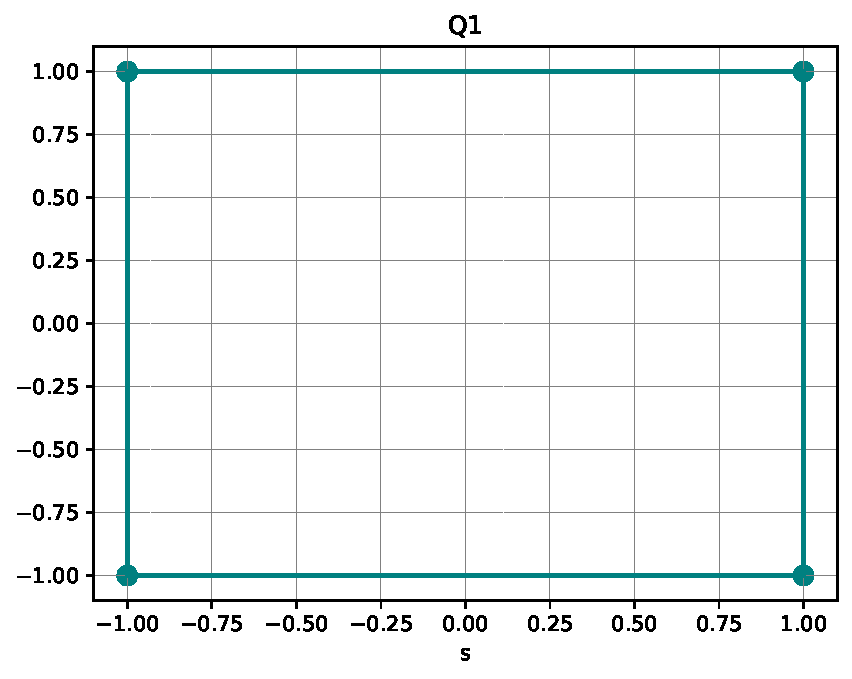
\includegraphics[width=3cm]{python_codes/fieldstone_120/spaces/Q1_nodes}
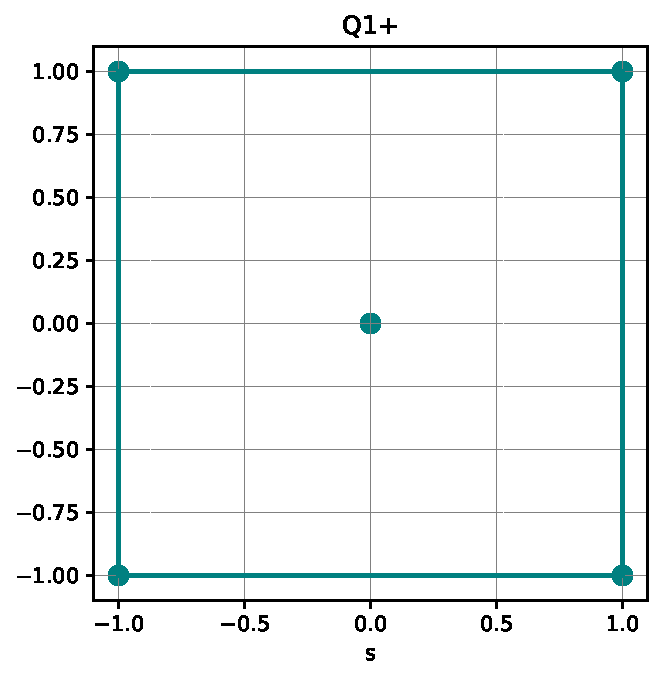
\includegraphics[width=3cm]{python_codes/fieldstone_120/spaces/Q1+_nodes}
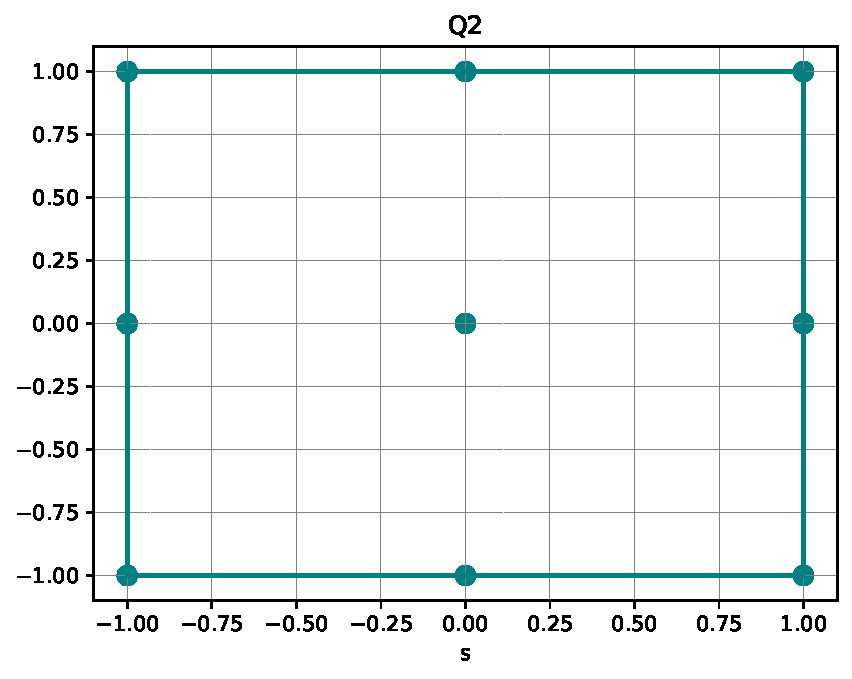
\includegraphics[width=3cm]{python_codes/fieldstone_120/spaces/Q2_nodes}
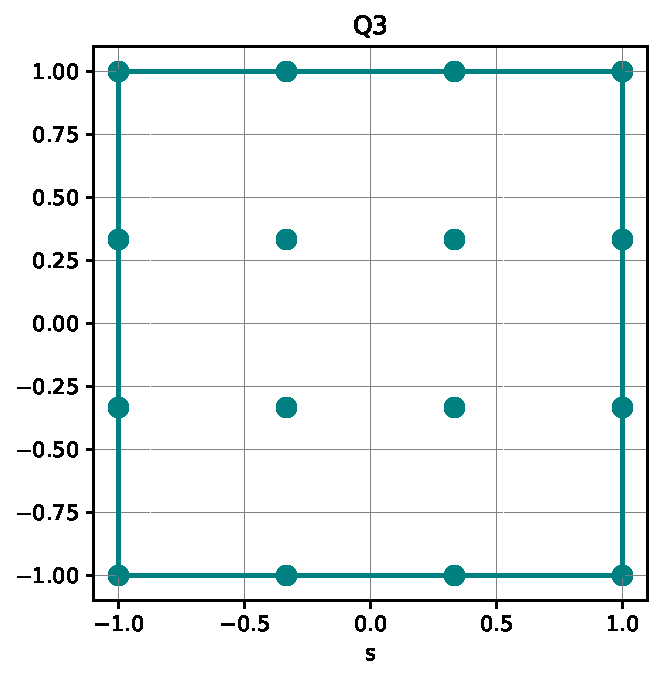
\includegraphics[width=3cm]{python_codes/fieldstone_120/spaces/Q3_nodes}
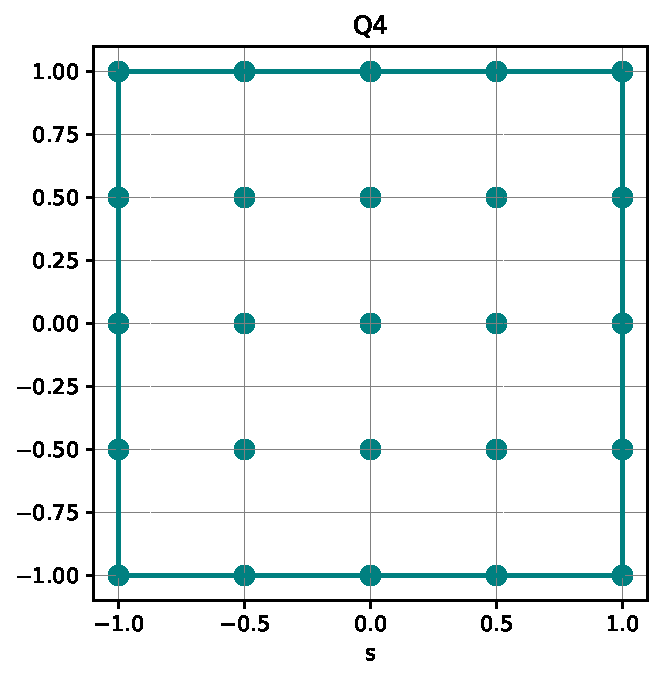
\includegraphics[width=3cm]{python_codes/fieldstone_120/spaces/Q4_nodes}

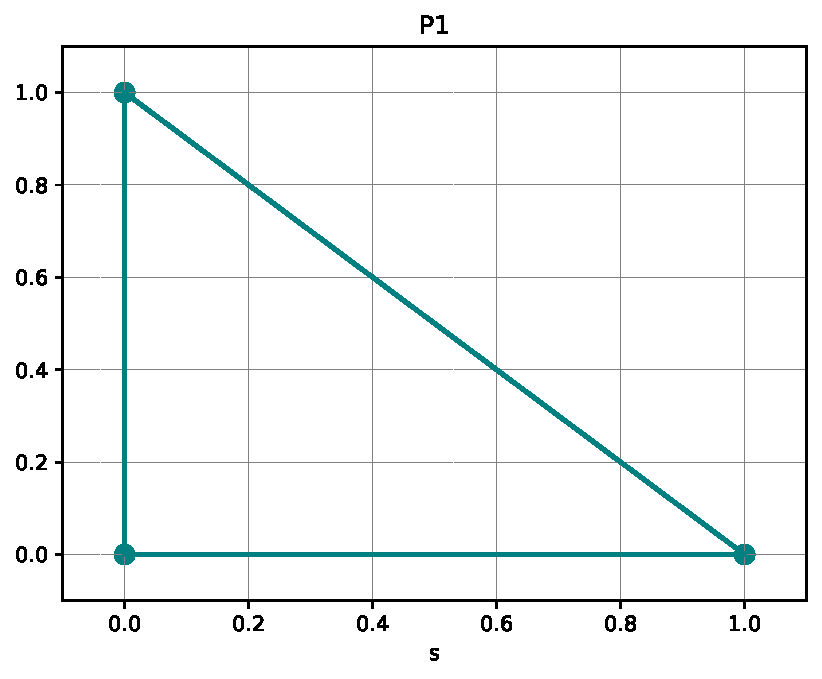
\includegraphics[width=3cm]{python_codes/fieldstone_120/spaces/P1_nodes}
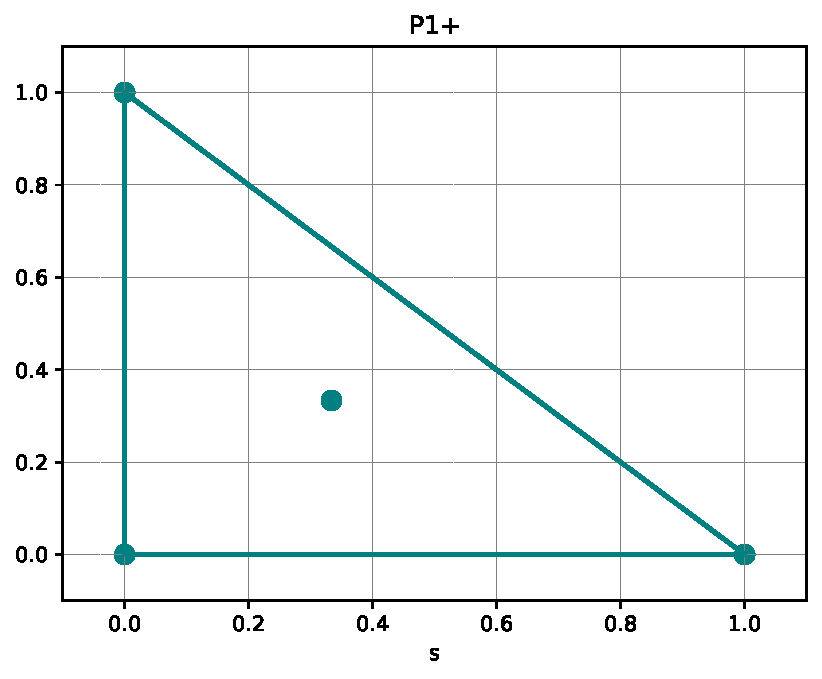
\includegraphics[width=3cm]{python_codes/fieldstone_120/spaces/P1+_nodes}
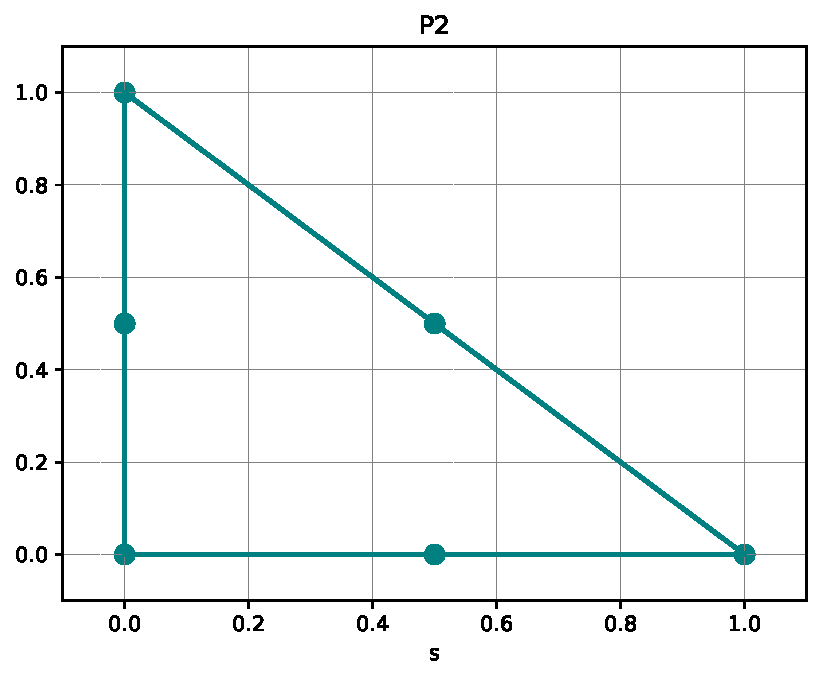
\includegraphics[width=3cm]{python_codes/fieldstone_120/spaces/P2_nodes}
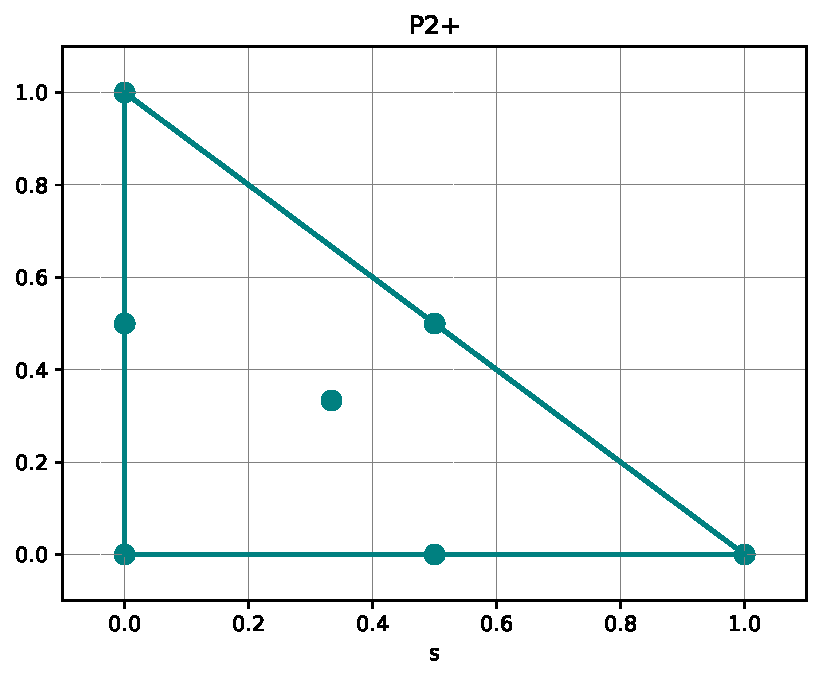
\includegraphics[width=3cm]{python_codes/fieldstone_120/spaces/P2+_nodes}
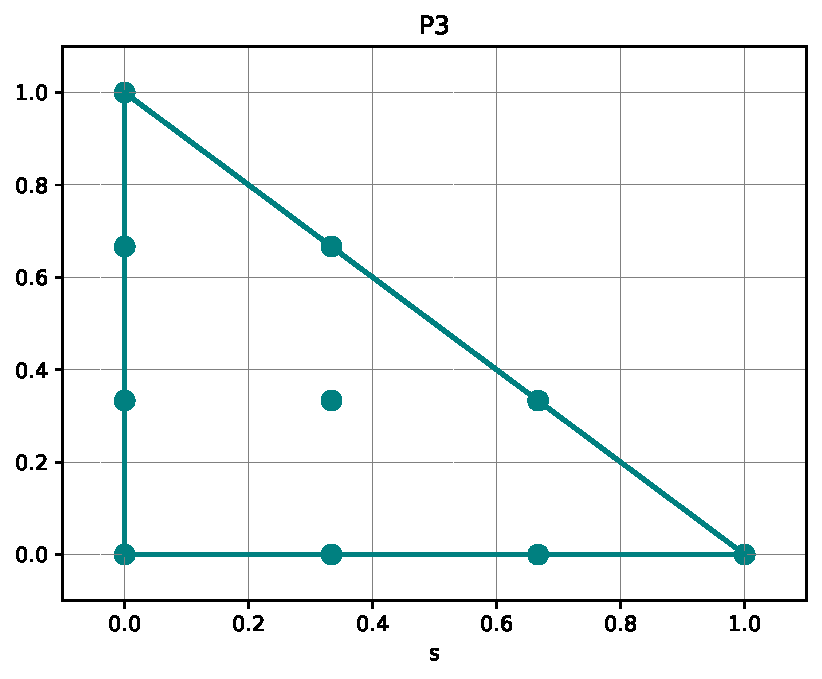
\includegraphics[width=3cm]{python_codes/fieldstone_120/spaces/P3_nodes}

mesher: Q0,Q1,Q2,Q3,Q4, P0,P1,P2   missing P1+, P2+, Q1+

\begin{tabular}{ccccccccccc}
      & Q1P0 & Q1Q1 & Q2Q1 & Q3Q2 & Q4Q3 & Q1+Q1 & P1P0 & P2P1 & P3P2 & P2+P1 & P1+P1 \\
\hline
areas  &  &&&&&&&&& \\ 
D\&H   &  \\
errors &  \\
vrms   &  \\
\hline
\end{tabular}

